\documentclass[DIV=12, ngerman, fontsize=12pt, parskip=half]{scrreprt}

\usepackage[utf8]{inputenc}
\usepackage[ngerman]{babel}
\usepackage[T1]{fontenc}
\usepackage{lmodern}
\usepackage{microtype}
\usepackage{graphicx}
\usepackage{csquotes}
\usepackage[onehalfspacing]{setspace}
\usepackage{tabularx}
\usepackage{mathtools}
\usepackage{amsmath}
\usepackage{amssymb}
\usepackage{float}
\usepackage{array}
\usepackage{subcaption}
\usepackage{bbold}
%\usepackage{subfig}
\clubpenalty10000
\widowpenalty10000

\begin{document}
	
	\setcounter{chapter}{1-1}
	
	\begin{center}
		
		\huge
		\textbf{Machine Learning I - Report: Exercise Sheet 1}
		
	\end{center}
	
	%\begin{figure}[h]
	%\centering
	%\includegraphics[width=3.25in]{UniRegensburgLogo}
	%\end{figure}
	
	
	\begin{center}
		\LARGE
		\textbf{Johannes Groß}
		
		\textbf{Leonard Bleiziffer}	
		
	\end{center}
	\vspace{5cm}
	\begin{center}
		\LARGE		
		\textbf{15.01.2020}
		
	\end{center}
	\thispagestyle{empty}
%	\tableofcontents 
	\thispagestyle{empty}
	
	\vspace{4cm}
	
	{\let\clearpage\relax \chapter{Maximum Likelihood}}
	The Maximum Likelihood (ML) estimates for mean and covariance is found for different data sets. In the second part of this task, ML estimates are used to perform a classification.
	
	\section{ML Estimates}
	The Gaussian distribution with mean $\mu  = [2,-2]^T$ and covariance $c = \big(\begin{smallmatrix}
		0.9 & 0.2\\
		0.2 & 0.3
	\end{smallmatrix}\big)$
	is used to generate two datasets with 50 and 5000 samples, respectively. For each data set the ML estimates for mean and covariance are calculated. The following plots illustrate the difference in the quality of the estimates for the mean:
	
	\begin{figure}[H]
	\begin{center}
		\begin{minipage}[t]{0.4\textwidth}
			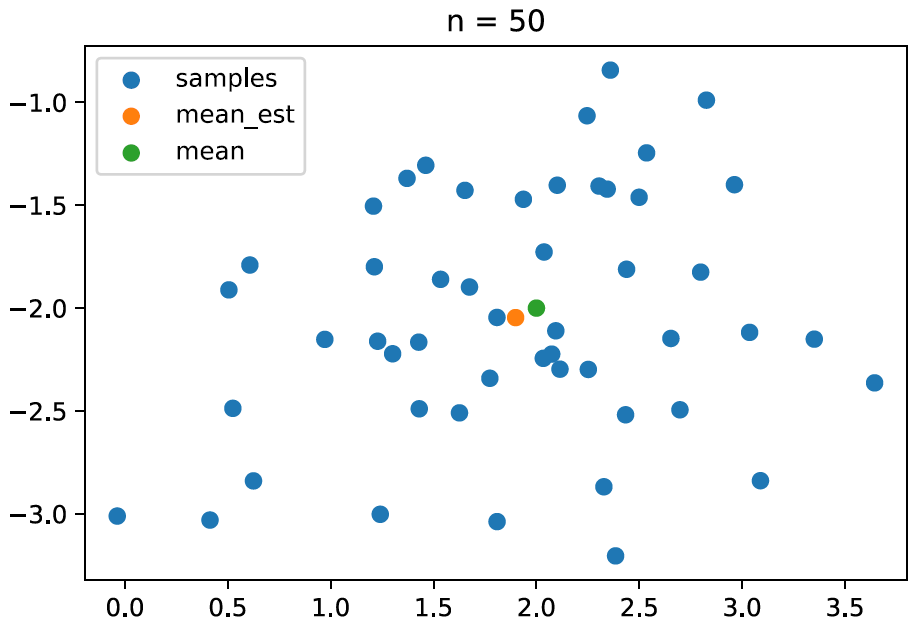
\includegraphics[width=\textwidth]{Task1_Mean_50_png}
		\end{minipage}
		\begin{minipage}[t]{0.4\textwidth}
			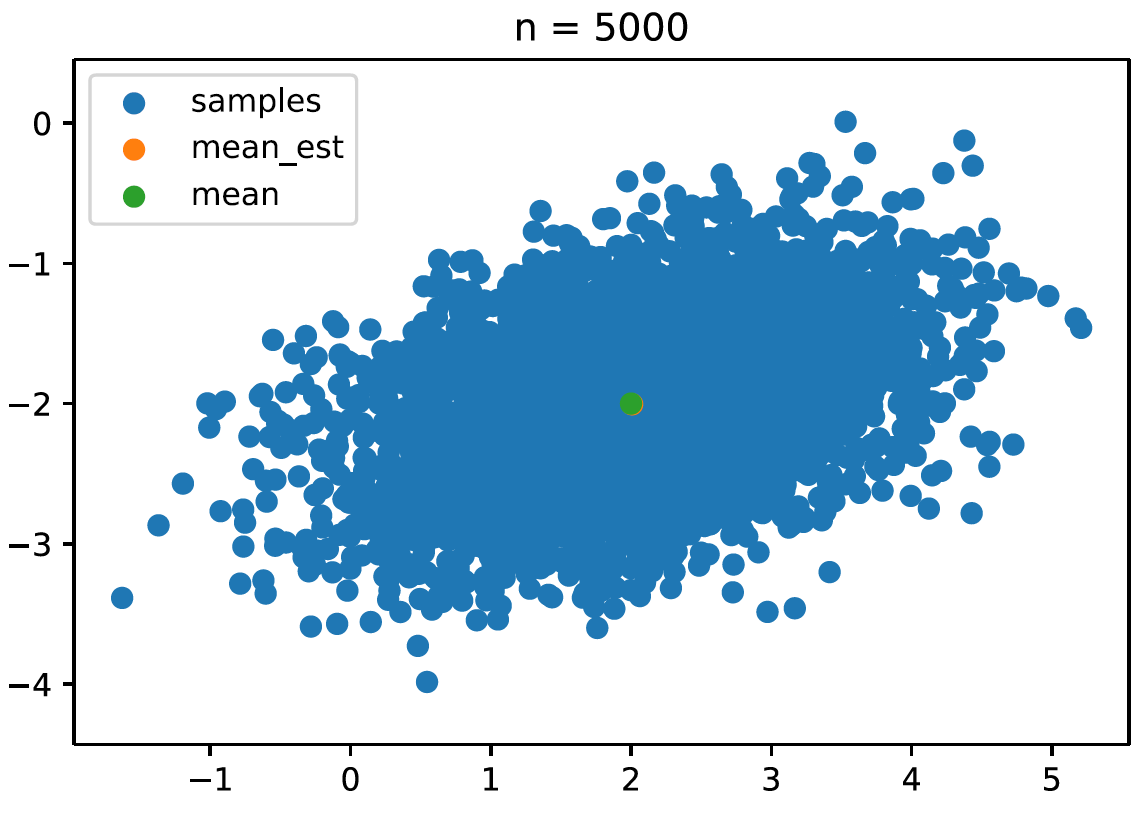
\includegraphics[width=\textwidth]{Task1_Mean_5000_png}
		\end{minipage}
	\end{center}
	\end{figure}

	The difference in quality can also be observed in the l2-distance to the exact mean of the distribution:
	\begin{align*}
		\mu_{50} = [1.899, -2.046]^T \quad \mu_{5000} = [2.008, -2.005]^T  
	\end{align*} 

	\begin{table}[H]
	\begin{center}	
		\begin{tabular}{|l|l|l|}
			\hline
			& 50 & 5000 \\
			\hline
			l2-distance & 0.1112   & 0.0092   \\
			\hline
		\end{tabular}
	\end{center}
	\end{table}

	While the estimates of the mean improve by two orders of magnitudes with respect to the l2-distance, the estimate of the covariance matrix improves by one order of magnitude with respect to the frobenius-distance, when increasing the number of samples from 50 to 5000:
	\begin{align*}
		c_{50} = \begin{pmatrix}			
					0.6539 & 0.1084\\
					0.1084 & 0.3500
				 \end{pmatrix}
		\quad 
		c_{5000} = \begin{pmatrix}			
					0.8855 & 0.1972\\
					0.1972 & 0.2946
					\end{pmatrix}
	\end{align*} 

	\begin{table}[H]
	\begin{center}	
		\begin{tabular}{|l|l|l|}
			\hline
			& 50 & 5000 \\
			\hline
			frob-distance & 0.2826   & 0.0160   \\
			\hline
		\end{tabular}
	\end{center}
	\end{table}
	
	
	\section{ML Classification}
	Using Maximum Likelihood, a classification task with three different classes was performed. All the samples had the same probability of $p(x \in k) = \frac{1}{3}$ to be drawn from class $k = 1,2,3$. The samples of the three classes are drawn from Gaussian distributions with different means, but a common covariance matrix. A training ($Train$) and a testing ($Test$) data set with 1000 samples each was created. \\
	 The samples in $Train$ were used to calculate the ML estimates for the mean and covariance. Then, the points in $Test$ were classified by calculating the l2-distance to each mean $\mu_k$ and assigning it to the class with the smallest distance. In order to quantify the quality of the classification, the fraction of correct assignments was determined. All of this was done for a diagonal and non-diagonal covariance matrix.
	
	\begin{figure}[H]
	\begin{center}
		\begin{minipage}[t]{0.4\textwidth}
			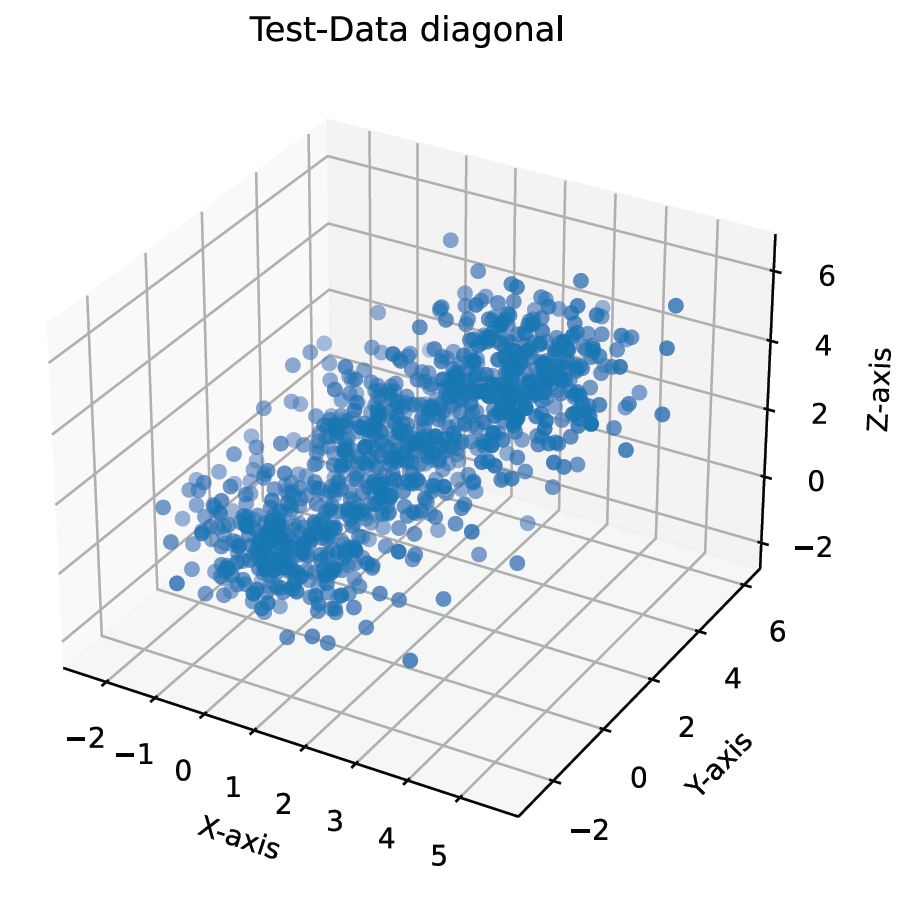
\includegraphics[width=\textwidth]{Task1_TestData_diag_png}
		\end{minipage}
		\begin{minipage}[t]{0.4\textwidth}
			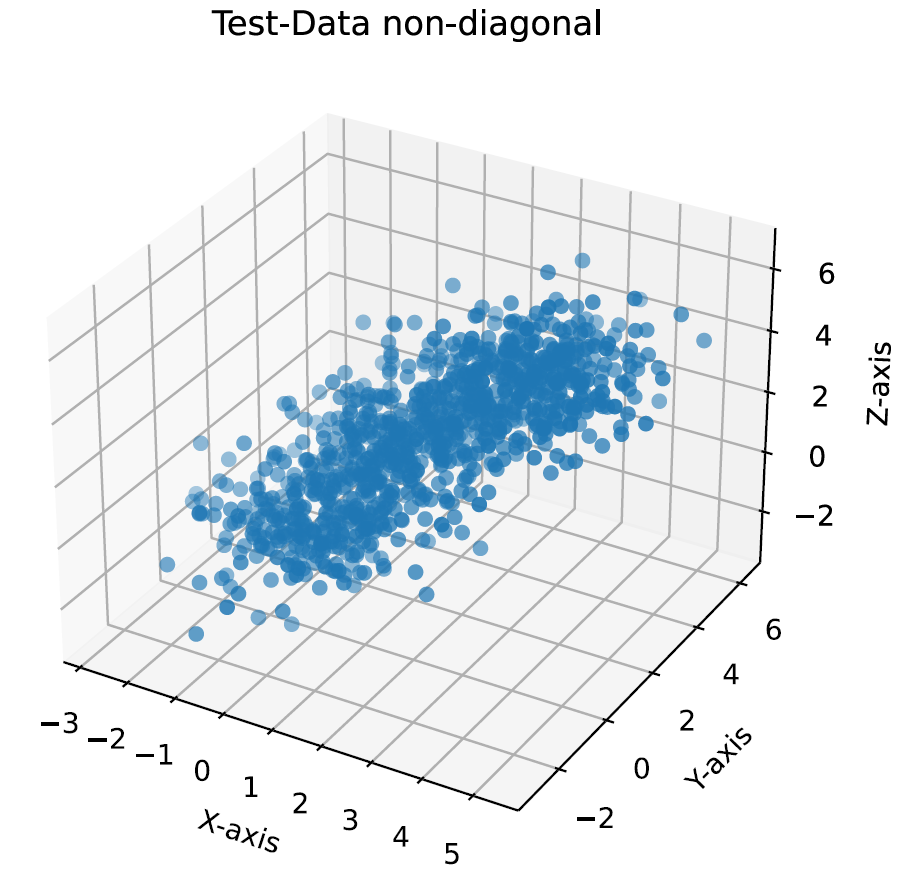
\includegraphics[width=\textwidth]{Task1_TestData_non_diag_png}
		\end{minipage}
	\end{center}
	\end{figure}

	It can be observed in the plots that the classes in the data generated with the diagonal covariance are more separated than in the non-diagonal case. This is also reflected in the ability of the ML-classifier to assign the samples to the correct class. The accuracy differs by $4\%$:
	
	\begin{table}[H]
	\begin{center}	
		\begin{tabular}{|l|l|l|}
			\hline
			& diagonal & non-diagonal \\
			\hline
			fraction of correct assignment & 0.9439   & 0.9039      \\
			\hline
		\end{tabular}
	\end{center}
	\end{table}

	
	
	{\let\clearpage\relax \chapter{Expectation Maximization}}
	In this task, the EM algorithm is applied and studied for different Gaussian mixture distributions:
	\begin{align*}
		p(x) = \sum_{k=1}^{K}P_k \cdot p(x|\Phi_k)
	\end{align*}

	
	\section{Estimating Parameters}
	600 samples were drawn from the a Gaussian mixture model with the following parameters: 
	\begin{align*}
		K = 3, \quad \mu_1 = [1,1]^T, \quad \mu_2 = [3,3]^T, \quad \mu_3 = [2,6]^T, \quad c_1 = 0.1 \cdot \mathbb{1},\\ \quad c_2 = 0.2 \cdot \mathbb{1}, \quad c_3 = 0.3 \cdot \mathbb{1}, \quad P_1 = 0.4, \quad P_2 = 0.4, \quad P_2 = 0.2
	\end{align*}
	This results in a distribution of samples shown below, where the mean estimates were determined with the EM algorithm using kmeans as the initialization method:
	
	\begin{figure}[H]
	\begin{center}
		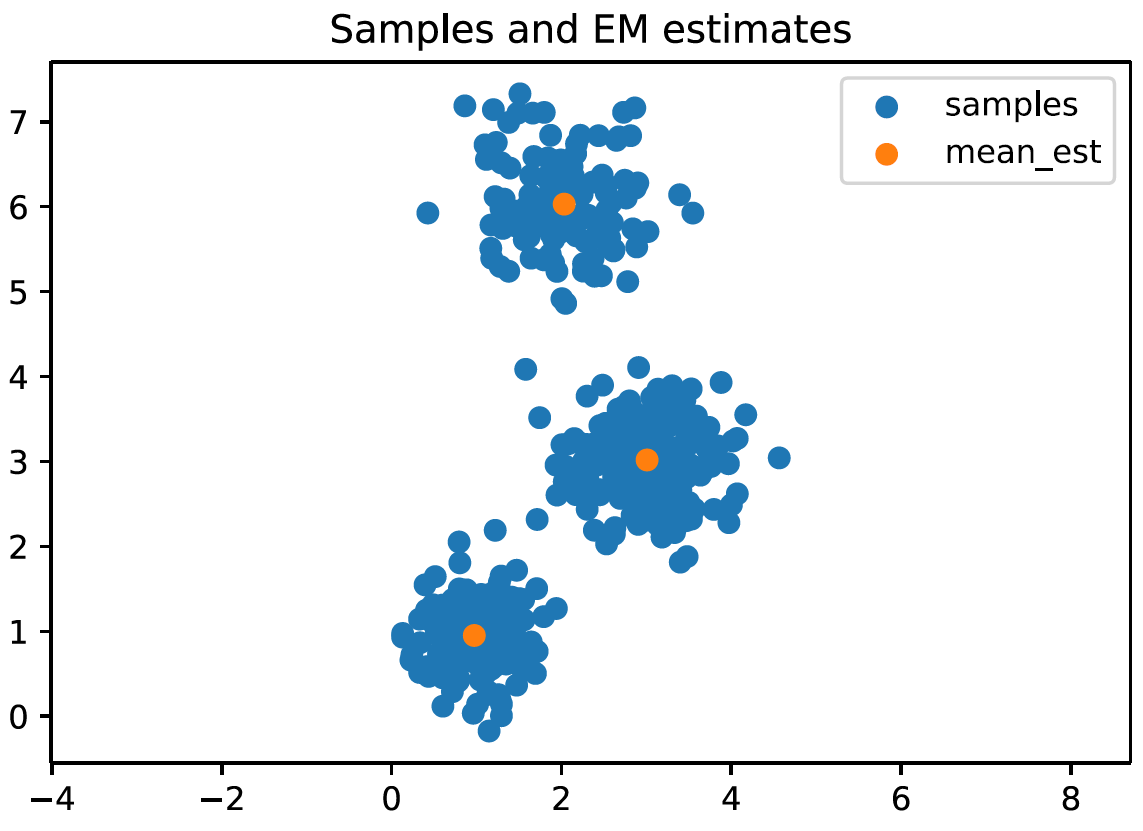
\includegraphics[scale=0.4]{Task2_TestData_Mean_Est_png}
	\end{center}
	\end{figure}

	The following table shows the errors on the different parameters. For the weights and covariances, the error was calculated as the absolute difference between the true value and the estimate (covariance: factor before identity-matrix). The error on the means is given by the l2-distance. No significant differences were found between the three classes:
	
	\begin{table}[H]
	\begin{center}	
		\begin{tabular}{|l|l|l|l|}
			\hline
			& class 1  & class 2  & class 3  \\ \hline
			weight\_error     & 4.30e-05 & 7.83e-04 & 7.40e-04 \\ \hline
			mean\_error       & 5.59e-02 & 1.94e-02 & 4.42e-02 \\ \hline
			covariance\_error & 1.68e-03 & 1.09e-03 & 4.56e-03 \\ \hline
		\end{tabular}
	\end{center}
	\end{table}
	
	\section{Varying Initial Parameters}
	Then, the performance of EM was tested by using two different sets of initial parameters and observing the results. The first set of parameters were:
	\begin{align*}
		K = 3, \quad \mu_1 = [0,2]^T, \quad \mu_2 = [5,2]^T, \quad \mu_3 = [5,5]^T, \\ c_1 = 0.15 \cdot \mathbb{1}, \quad c_2 = 0.27 \cdot \mathbb{1}, \quad c_3 = 0.4 \cdot \mathbb{1}, \quad P_1 = P_2 = P_3 = 0.33
	\end{align*}
	And the second set:
	\begin{align*}
	K = 2, \quad \mu_1 = [1.6,1.4]^T, \quad \mu_2 = [1.4,1.6]^T, \\ c_1 = 0.2 \cdot \mathbb{1}, \quad c_2 = 0.4 \cdot \mathbb{1}, \quad P_1 = P_2 = 0.5
	\end{align*}	

	Below, the results for the two sets of initial parameters are shown. With the first set of parameters, the algorithm converges to the correct results with similar errors as before with kmeans used as an initialization method. \\
	Of course, EM had no chance to determine good estimates with the second set of initial parameters, as it tried to find estimates for two instead of three classes. However, the mean of class 1 was estimated quite precisely and the second mean was estimated to lie between classes 2 and 3. Furthermore, it is interesting to note that the estimated weights and covariances seem to indicate that classes 2 and 3 where taken to be one class by the EM algorithm. \\
	After further experimentation with the initial parameters, the following can be summarized for the EM algorithm: if the number of classes is not set correctly initially, the results will deviate greatly from the exact parameters; the other initial parameters have to be roughly in the right ballpark, whilst the EM seems to be most sensitive to the initialization of the means. 

	\begin{figure}[H]
		\begin{minipage}[b]{0.5\textwidth}
			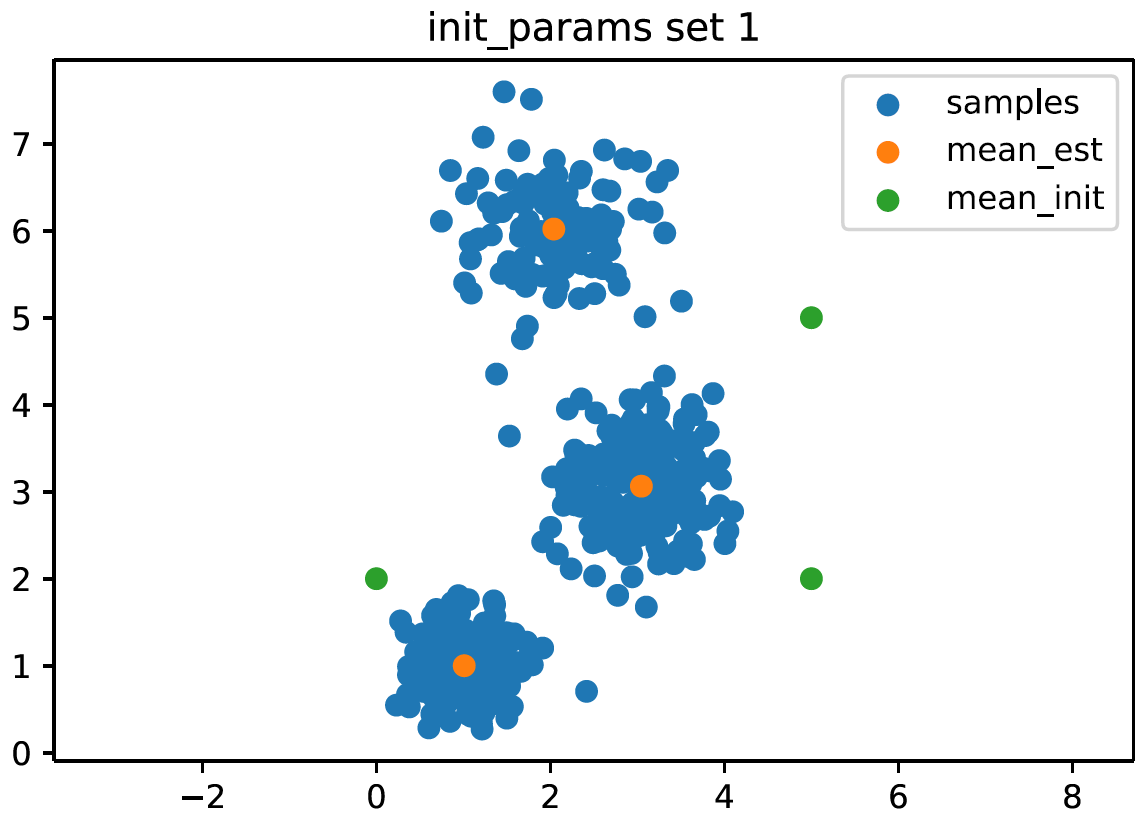
\includegraphics[width=\textwidth]{Task2_initparams_set1_png}
		\end{minipage}
		\begin{minipage}[b]{0.5\textwidth}
			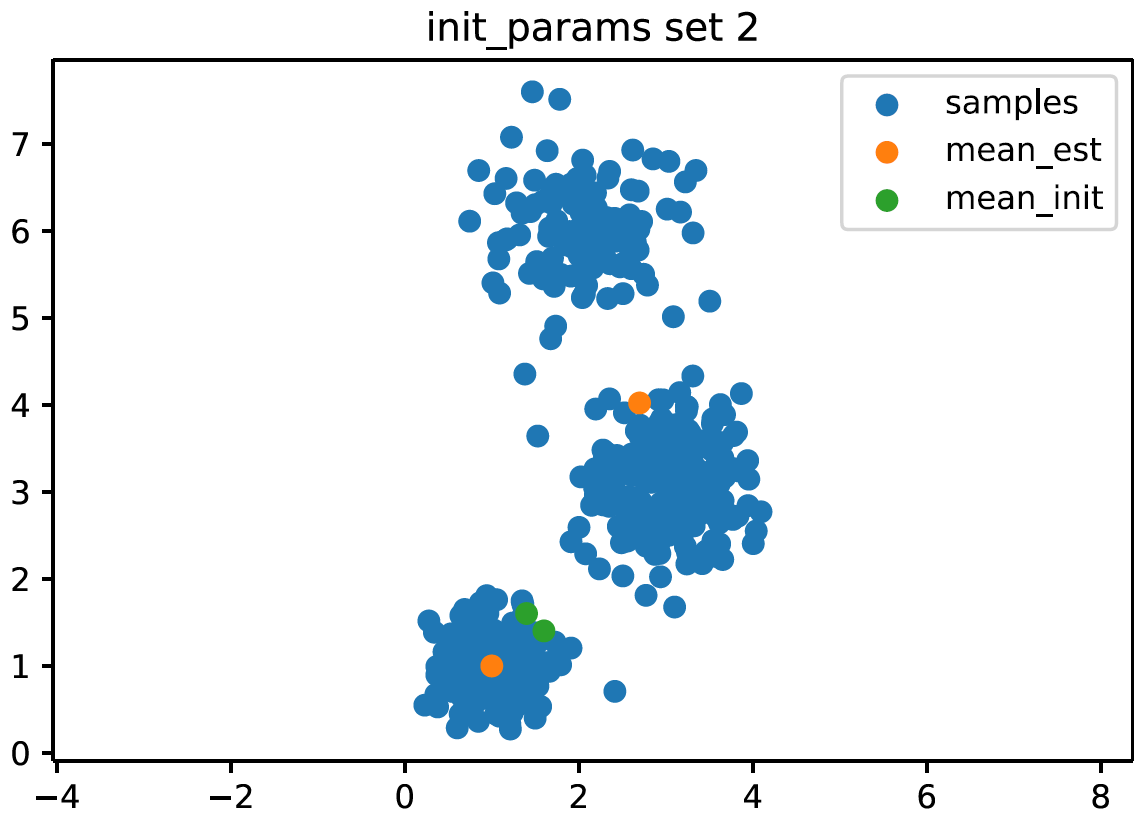
\includegraphics[width=\textwidth]{Task2_initparams_set2_png}
		\end{minipage}
	\end{figure}

	\vspace{3cm}
	

	{\let\clearpage\relax \chapter{Clustering}}
	
	A data set $Train$ was created, that consists $N = 1000$ samples grouped into four equally sized classes. Each class is described by a Gaussian distribution with the following parameters:
	\begin{align*}
		\mu_1 = [0,0]^T, \quad \mu_2 = [10,0]^T, \quad \mu_3 = [0,6]^T, \quad \mu_4 = [9,8]^T, \\
		c_1 = \mathbb{1}, \quad 
		c_2 = \begin{pmatrix}			
			1 & 0.2\\
			0.2 & 1.5
		\end{pmatrix}, \quad 
		c_3 = \begin{pmatrix}			
			1 & 0.4\\
			0.4 & 1.1
		\end{pmatrix}, \quad 
		c_4 = \begin{pmatrix}			
		0.3 & 0.2\\
		0.2 & 0.5
		\end{pmatrix}
	\end{align*}

	Now the K-means algorithm is applied to $Train$ with different initial parameters. First, only the number of initialized classes was varied. Obviously, the algorithm performed best in the case where the number of initialized classes matches the actual number of classes. In the case with three initialized classes, K-Means takes the classes 1 and 3 to be one, probably because they are closest together. In the last case, the algorithm splits class 2 in half, seemingly since it is spread the most (see covariance matrices).
	
	\begin{figure}[H]
	\begin{center}
		\begin{minipage}[t]{0.4\textwidth}
			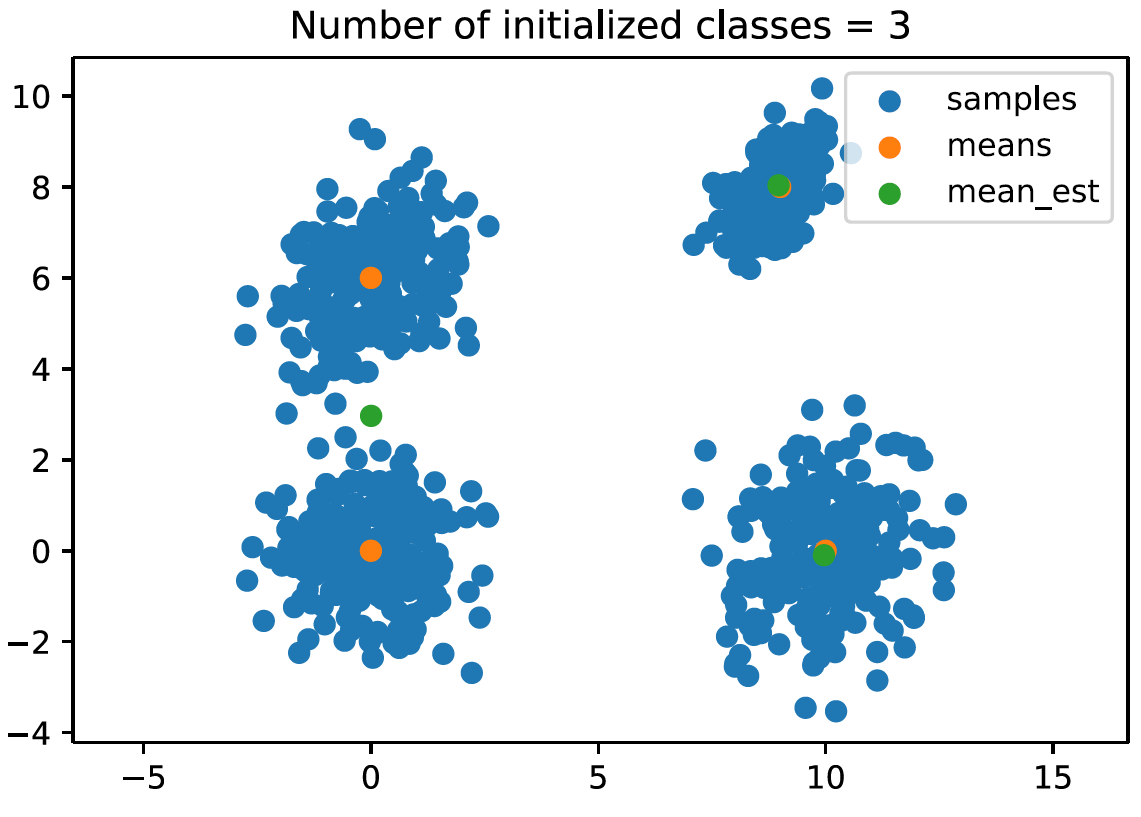
\includegraphics[width=\textwidth]{Task3_classes3_png}
		\end{minipage}
		\begin{minipage}[t]{0.4\textwidth}
			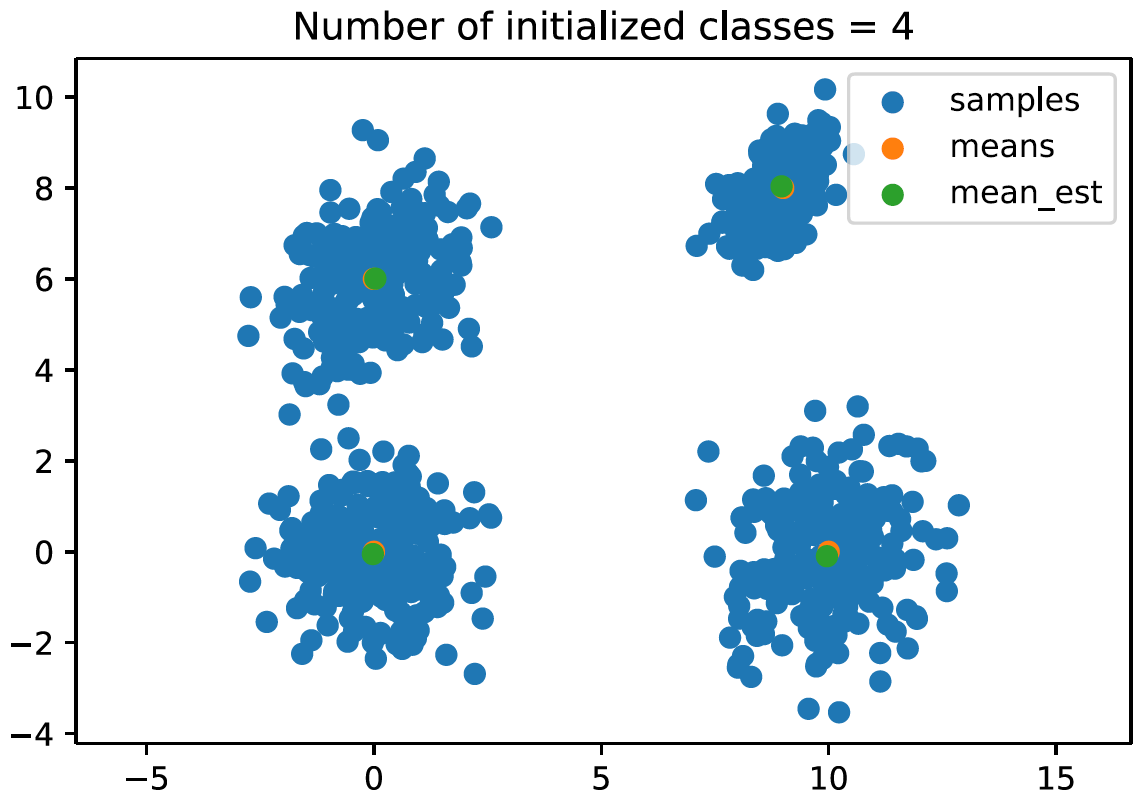
\includegraphics[width=\textwidth]{Task3_classes4_png}
		\end{minipage}
		\begin{minipage}[b]{0.4\textwidth}
		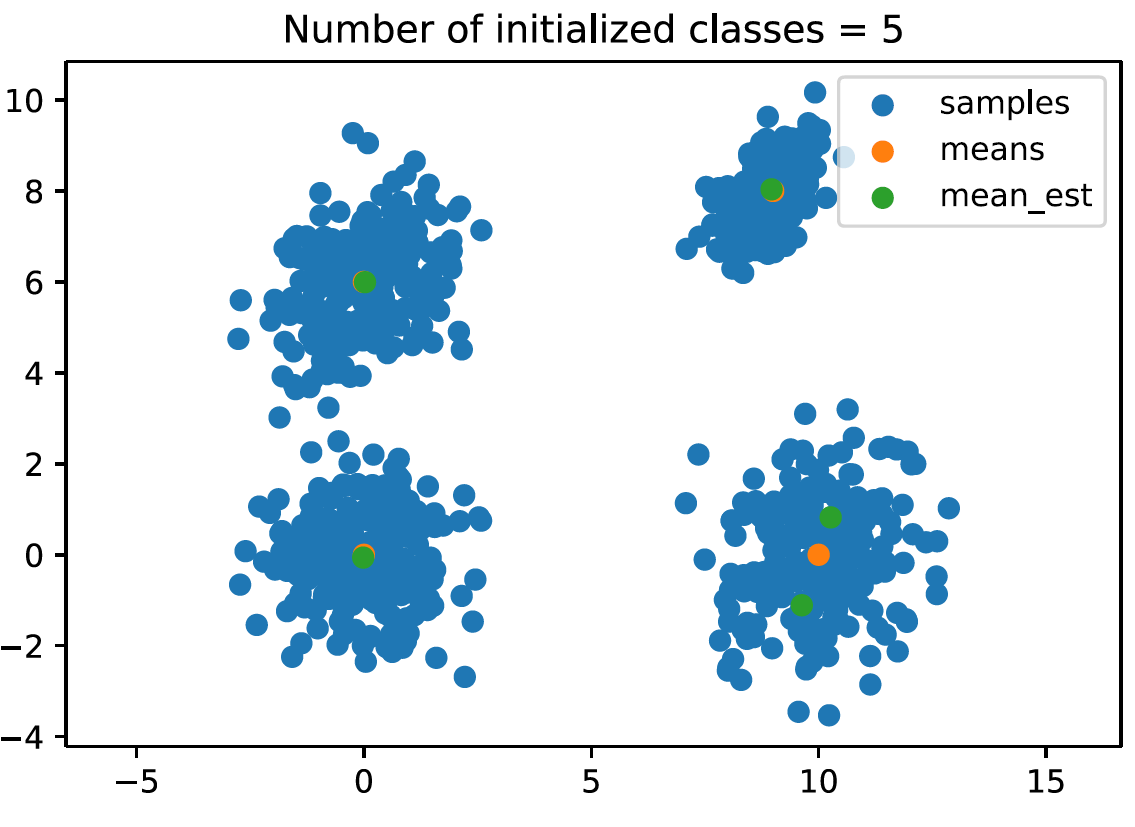
\includegraphics[width=\textwidth]{Task3_classes5_png}
		\end{minipage}
	\end{center}
	\end{figure}

	Furthermore, the algorithm was run two more times, with the correct number of classes initialized. Once, with the means initialized in the following way:

	\begin{align*}
		\mu_1 = [-2,-2]^T, \quad \mu_2 = [-2.1,-2.1]^T, \quad \mu_3 = [-2,-2.2]^T, \quad \mu_4 = [-2.1,-2.2]^T
	\end{align*}

	And another time with the first three means initialized randomly and the fourth as $\mu_4 = [30,30]^T$. 
	
	\begin{figure}[H]
		\begin{minipage}[t]{0.5\textwidth}
			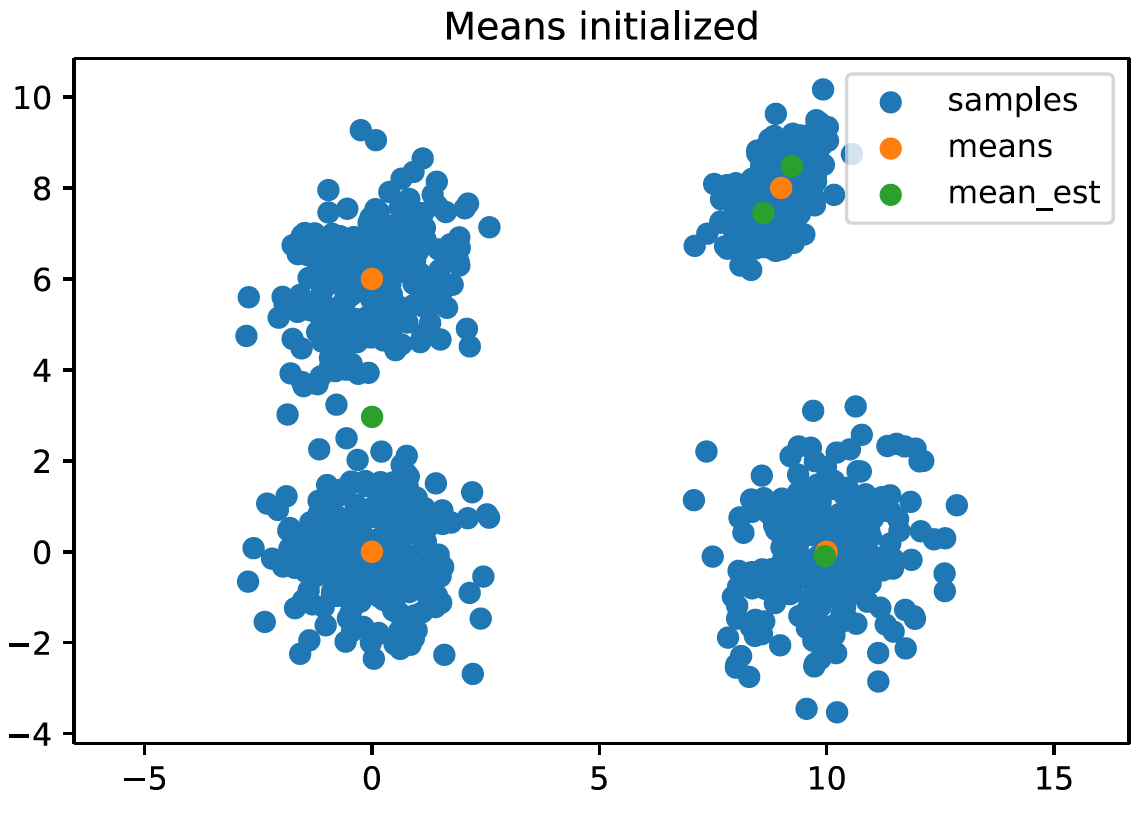
\includegraphics[width=\textwidth]{Task3_means_init4_png}
		\end{minipage}
		\begin{minipage}[t]{0.5\textwidth}
			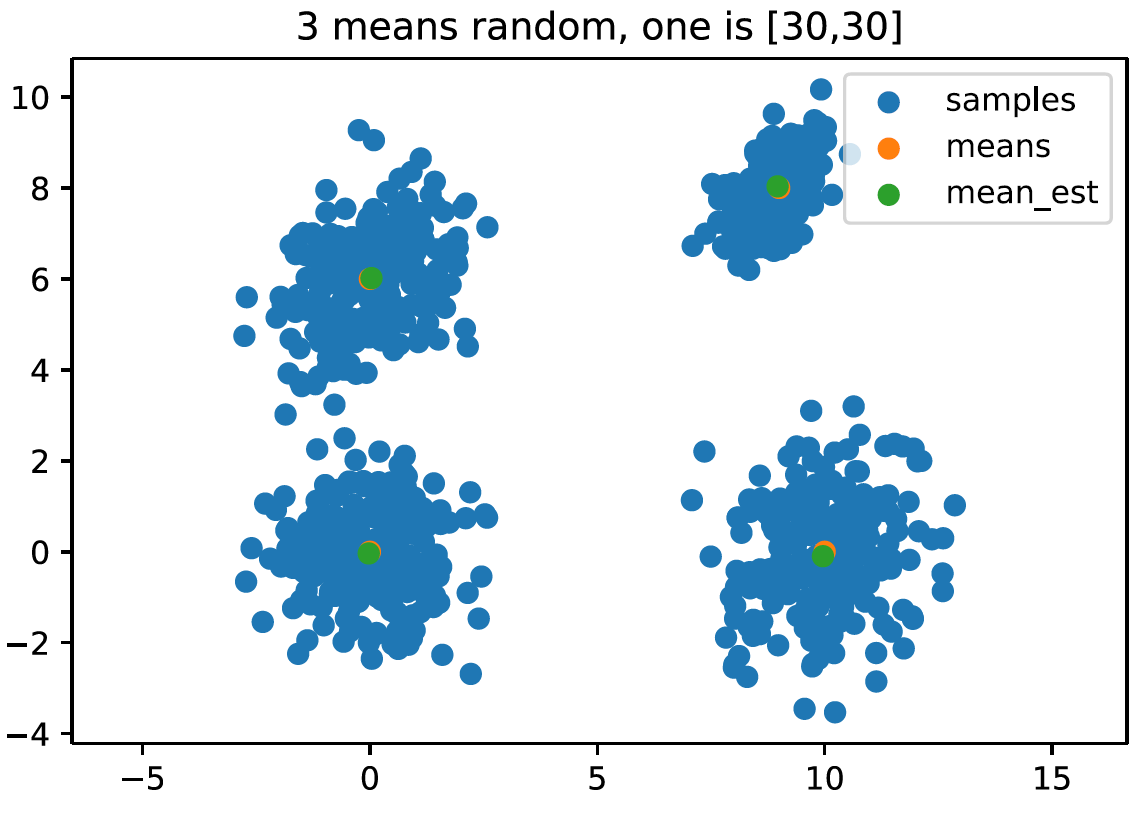
\includegraphics[width=\textwidth]{Task3_means_init1_png}
		\end{minipage}
	\end{figure}

	This shows that even when the number of classes is initialized correctly, the results depend highly on the initial means. On the other hand, it is interesting that K-means can sometimes handle one mean to be initialized completely wrong. However, in some runs of the algorithm (with different random means and the same fourth mean $\mu_4 = [30,30]^T$), it didn't converge correctly, supporting the statement that the results are highly dependent on the initial conditions.
	
	
\end{document}